\section{کاربرد های دیگر برنامه ریزی مسیر}
زمانی که محیط به گراف گسسته تبدیل شد، ما می توانیم الگوریتم های دیگری که راجب تئوری گراف
 هست استفاده کنیم تا مسیر حرکتی دلخواه رو برنامه ریزی کنیم ، برای مثال، پوشش کف با انجام
\rl{depth-first-search} 
  یا
\rl{breadth-first-search} 
 روی یک گراف جایی که هر راس اندازه ی ابزار پوشش ربات رو دارد.  پوشش
\rl{(coverage)}
فقط برای تمیز کردن سطح استفاده نمیشه و در جستوجوی های کامل فضای پیکربندی مثل شکل
\ref{fig:coverage}
استفاده میشه، نمایش داده شده.پیدا کردن مینیمم در این نمودار با استفاده از جستوجوی کامل مسئله ی سینماتیک معکوس انجام شده.
و  همچنین الگوریتم مشابه میتواند همه ی لینک های روی یک وبسایت را تا عمق دلخواه بدست آورد.
\begin{figure}[H]
\begin{center}
  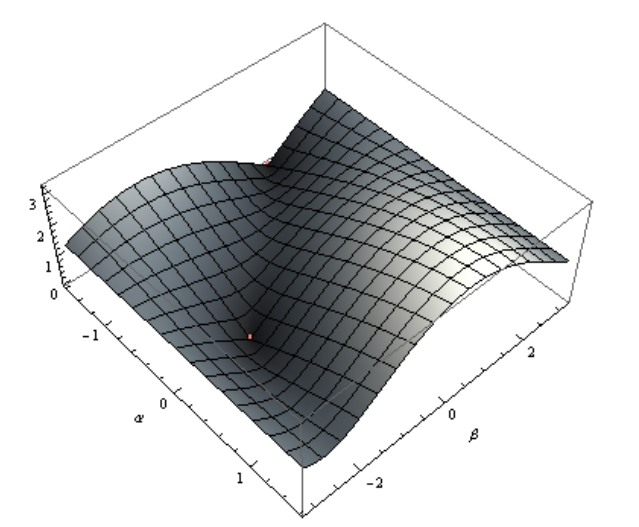
\includegraphics[ scale=0.5]{images/coverage.png}
  \caption{برنامه ریزی مسیر در مقیاس های طولی مختلف}
  \label{fig:coverage}
\end{center}
\end{figure}

انجام 
\rl{(DFS)}
 و
 \rl{(BFS)}
می تواند  مسیر های پوششی کارآمد را تولید کند، ولی به اندازه ی کافی بهینه نیست
 چون یه راس ممکن است دوبار دیده شود. یک مسیر که همه ی راس ها را به هم وصل کرده و از هر راس یک بار عبور کرده را با مسیر همیلتونی  می شناسند. یک مسیر همیلتونی که که به راس شروع برمیگردد را با دور همیلتونی میشناسند. این مسئله همچنین با نام فروشنده ی دوره گر نیز شناخته میشود و در این مسئله مسیر باید طوری حساب شود که از هر شهر فقط یکبار عبور شود و یک مسئله
\rl{\textbf{NP-complete}}
 است. 

